\documentclass[11pt]{article}

\usepackage{changepage} \usepackage{titlesec} \usepackage{titling}
\usepackage{lipsum} \usepackage{graphicx} \usepackage{subcaption}
\usepackage{float} \usepackage{listings} \usepackage{color}


% listing boxes
\usepackage[most]{tcolorbox}
\usepackage{caption}
\usepackage{courier}


% Use wide margins, but not quite so wide as fullpage.sty
\marginparwidth 0.5in \oddsidemargin 0.25in \evensidemargin 0.25in
\marginparsep 0.25in \topmargin 0.0in \textwidth 6in \textheight 8 in

\titleformat{\section} {\Large\bfseries} {} {0em} {}

\titleformat{\subsection} {\bfseries} {} {.0em} {}
%\titleformat{\subsection} {\bfseries} {\hspace{.1in}$\bullet$} {.7em} {}

\titleformat{\subsubsection} {\bfseries} {\hspace{.1in}$\bullet$
\hspace{.005in}} {0em} {}

\setlength{\parskip}{\baselineskip}% 
\setlength{\parindent}{0pt}%


\definecolor{dkgreen}{rgb}{0,0.6,0}
\definecolor{gray}{rgb}{0.5,0.5,0.5}
\definecolor{mauve}{rgb}{0.58,0,0.82}

%\lstset{frame=tb,
%  language=C,
%  aboveskip=3mm,
%  belowskip=3mm,
%  showstringspaces=false,
%  columns=flexible,
%  basicstyle={\small\ttfamily},
%  numbers=none,
%  numberstyle=\tiny\color{gray},
%  keywordstyle=\color{blue},
%  commentstyle=\color{dkgreen},
%  stringstyle=\color{mauve},
%  breaklines=true,
%  breakatwhitespace=true,
%  tabsize=3
%}

\lstdefinestyle{Cstyle}{
frame=tb,
  language=C,
  showstringspaces=false,
  columns=flexible,
  basicstyle={\small\ttfamily},
  numbers=none,
  numberstyle=\tiny\color{gray},
  keywordstyle=\color{blue},
  commentstyle=\color{dkgreen},
  stringstyle=\color{mauve},
  breaklines=true,
%  breakatwhitespace=true,
  tabsize=3
}

% Code environment. Does inherit from lstset settings thanks to style.
\newtcblisting[auto counter]{ccode}[2][]{%
    listing only,
    breakable,
    top=0.5pt,
    bottom=0.5pt,
    left=6mm,
    sharp corners,
    boxrule=0pt,
    bottomrule=1pt,
    toprule=1pt,
    enhanced jigsaw,
    listing options={
        style=Cstyle,
        numbers=left,
        numberstyle=\tiny,
    },
    lefttitle=0pt,
    coltitle=black,
    colbacktitle=white,
    % Crashes on long lstlisting lines. \the\baselineskip reports 12.0pt. 1.2 * 12.0 = 14.4
    %borderline north={1pt}{1.2\baselineskip}{dashed},
    borderline north={1pt}{14.4pt}{dashed},
    title={\GetTranslation{codeSnippet} \thetcbcounter:  #2},#1
}


\begin{document} \hfill\vbox{\hbox{Ahlquist, Ethan} \hbox{Delaplaine, Victor} \hbox{CPE 453, Section 01}
\hbox{Lab 2}	\hbox{\today}}\bigskip

   \centerline{\Large\bf Asgn 4: Minix Secret Driver}

\section{What to Turn In: }

\begin{adjustwidth}{.2in}{}{
\titlerule

      \begin{itemize}

         \item An overall architecture of the driver: How is it expected to
         function?\\  
      

         \item A detailed description of the driver implementation including:\\

            \begin{itemize}

               \item Your development environment: version of the Minix kernel
                  and type of installation(platform, native vs. bochs, qemu, or
                  VMware)\\

               \item A list of all files modified, and the modifications (along
                  with why such modification was necessary),\\

               \item The complete code of your driver.\\

            \end{itemize}

         \item A description of the driver’s behavior when running in the
            system.  If possible, include typescript or screenshot of the
            driver in action. (The screenshot is easy if you are running
            simulator, not easy if you are running a native installation.)\\

         \item A section listing problems encountered, solutions attempted,
            results obtained, and lessons learned as previous labs.\\

         \item Other things as necessary: Remember, the meta-goal here is to
            convince the reader of the report that you successfully implemented
            a Secret Keeper device, or, failing that, to convey what you did do
            and that you learned something useful.\\

      \end{itemize} 
}\end{adjustwidth}

\titlerule
\newpage

\section{Architecture}
\begin{adjustwidth}{.2in}{}{

   This driver is supposed to create restricted file, in the form of a drive
   driver. The reason, being that the user restriction is based on user-ID
   rather than the group-level. This makes it so that the number of people that
   are owners of the file are 0 or 1. 

   This makes sense why we label this device drive (secretKeeper), because it
   restricts access of the file to only the user who last wrote to the empty
   device, and they alone are able to read from it.

   For example:      

   
         \begin{adjustwidth}{.2in}{}{\tt service up /usr/src/drivers/secrets/secret -dev /dev/secret
         }\end{adjustwidth}

         This should start our driver as a service connected to {\tt /dev/secret}
         
         \begin{adjustwidth}{.2in}{}{\tt echo "Hello Person" > /dev/secret 
         }\end{adjustwidth}

         This gives the user who ran this command exclusive access to read from {\tt /dev/secret}

         
         \begin{adjustwidth}{.2in}{}{\tt su victor \\ cat /dev/secret
         }\end{adjustwidth}

         This should not work, because you are no longer the user that wrote to {\tt /dev/secret}

         \begin{adjustwidth}{.2in}{}{\tt su root \\ cat /dev/secret \\ Hello Person
         }\end{adjustwidth}

         This time it worked because you are the right user

}\end{adjustwidth}


\section{Implementation}
\begin{adjustwidth}{.2in}{}{

   \subsection{Development Environment}
   
      We had only one Minix machine able to connect to the internet. So we
         could only work from one computer or through ssh.

      On both of our computers used the {\tt Virtual Box} virtualizer.

   \subsection{Files Modified:}


      /usr/src/drivers/hello/hello.c
      \begin{itemize}
         \item[--] This code was used as the basis for our secret driver
      \end{itemize}
 

      /etc/system.conf
         \begin{itemize}
            \item[--] Tells the kernel of a new valid service type (secret)
            \item[--] Tells the OS knows what the service should have access to, and what permissions it needs
      \end{itemize}

      

      /usr/src/includes/sys/ioctl.h
      \begin{itemize}
         \item[--] Changing ioctl includes allows it to have acess to the secret dirver that are needed to use secret driver with other programs.
      \end{itemize}

      
      /usr/src/includes/sys/ioc\_secret.h
      \begin{itemize}
         \item[--] Gives the secret driver a unique key ID for programs, being 'K'
      \end{itemize}
      

   \newpage
   %\subsection{Code of Driver}
   {\bf Secret.c Source Code:}
   \lstset{style=Cstyle}
   \lstinputlisting[language=C]{./code/secret.c} 

   \bigskip

   {\bf Makefile:}
   \lstinputlisting[language=C]{./code/Makefile} 

}\end{adjustwidth}


\newpage

\section{Behavior}
\begin{adjustwidth}{.2in}{}{

      \vspace{-5mm}

      In order to display functionality under different test cases, we placed
      print statements in out code, to show what was being done behind the
      scenes. These are some such outputs:


      {\tt \bf Nico's Sample Run: }

         \vspace{-5mm}
         \begin{itemize} 
         
            \item Provided by professor

            \item Tests the driver's ability to tell user possession of driver.  

            \item Tests driver's ability to tell wither it is full or empty,
               and respond appropriately.

         \end{itemize}


      \begin{figure}[H]
         \centering
         \fbox{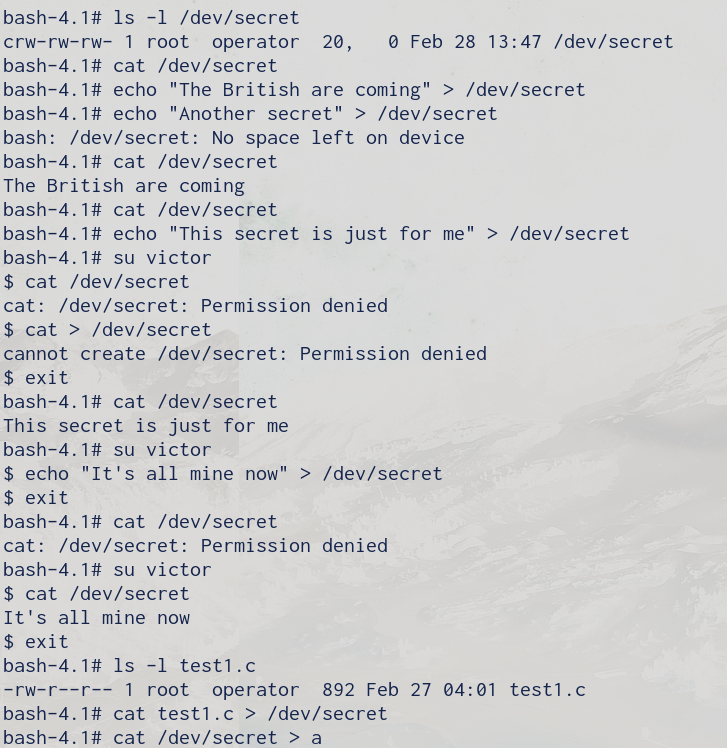
\includegraphics[width=.9\linewidth]{images/nicoTestInv.png}}
         \caption{Nico's Sample Run}
         \label{fig:latex}
      \end{figure}

      \newpage

      {\tt \bf BigMessage: }

         \vspace{-5mm}
         \begin{itemize} 
         
            \item Provided by professor

            \item Tests edge case where the driver is given a message larger
            than it can store

         \end{itemize}

      \begin{figure}[H]
         \centering
         \fbox{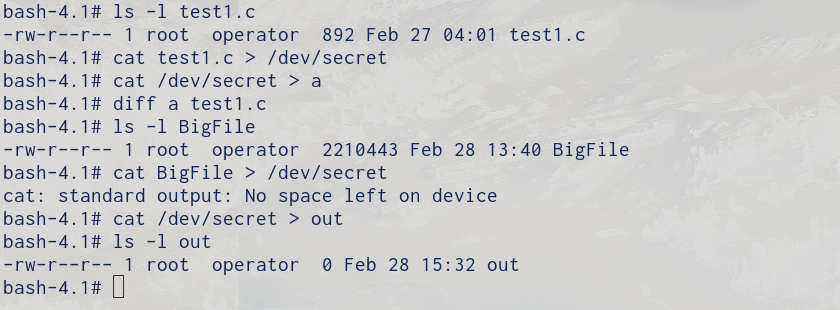
\includegraphics[width=.9\linewidth]{images/BigFileInv.png}}
         \caption{Service Update Test Output}
         \label{fig:latex}
      \end{figure}


      {\tt \bf Owner Behavior: }

         \vspace{-5mm}
         \begin{itemize} 
         
            \item One of our tests

            \item Again, tests the driver's correct response to user IDs 

            \item Tests using print-statements inside the driver source code

            \item Code directly changes the uid of the process, to fool the driver

            \item In the end, changing the uid will allow the driver to be read from

         \end{itemize}

      \begin{figure}[H]
         \centering
         \fbox{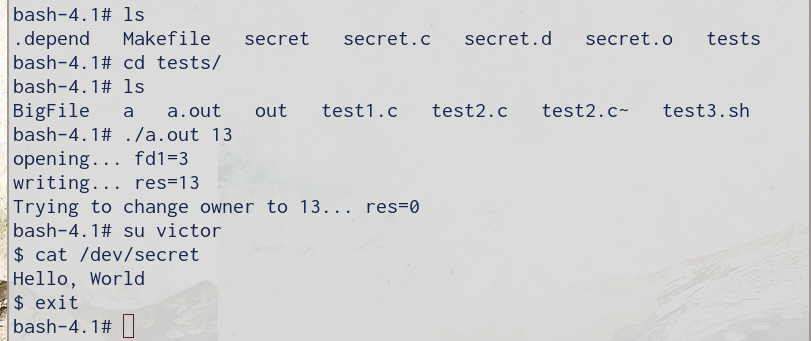
\includegraphics[width=.9\linewidth]{images/OwnerBehaviorInv.png}}
         \caption{Service Update Test Output}
         \label{fig:latex}
      \end{figure}

      {\tt \bf Refresh Secret: }

         \vspace{-5mm}
         \begin{itemize} 
         
            \item One of our tests

            \item Tests {\tt service refresh secret}

            \item Tests the ability of the driver to Refresh 

            \item The {\tt "Hello World"} shows that driver {\tt open()} protocol is being run

            \item The {\tt "Hey, I've just been restarted"} shows that the
            reincarnation code is being run

         \end{itemize}

      \begin{figure}[H]
         \centering
         \fbox{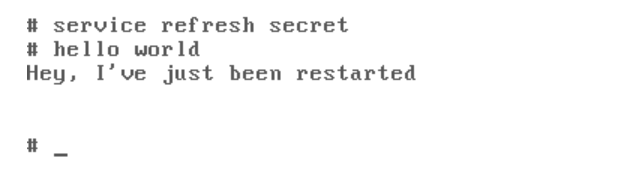
\includegraphics[width=.9\linewidth]{images/RefreshSecretInv.png}}
         \caption{Service Update Test Output}
         \label{fig:latex}
      \end{figure}

      \vspace{-5mm}
      {\small NOTE: this image looks different, because this was captured via the
               Virtual Box screen Capture, whereas the other Screenshots are
               taken from an ssh terminal.}



}\end{adjustwidth}


\section{Problems Encountered}
   
   \begin{itemize} 
      
      \item Sharing Code Bases, since Minix is harder to work with than a normal machine.

         We also had the addeed difficulty that one of our machine's Minix could not connect to the internet. 

      \item understanding {\tt service(8)}

      \item Understanding how Minix drivers worked

      \item Broken Makefile

      \item Debugging issues

   \end{itemize}


\section{Solutions Developed}

   \begin{itemize}

      \item Sharing code required us to ssh into a VirtualBox Minix machine.
      This was complicated with the fact that ssh-ing directly into Minix from
      my Linux caused problems. \\

      To solve this, we found that first ssh-ing into the partner's Linux, and
      from there ssh-ing into Minix worked the best.\\

      Lastly, for sharing all the code, it was fortunate that the code could be
      pushed to github from Minix. \\

      \item {\tt service(8)} took very long to understand. The man page was not very specific about what paths should be used where, and what the commands where supposed to do.

      We spent time reading man pages, and trying {\tt service(8)} in different ways with the hello driver. \\

      Eventually, by bruit force we found out how to use it. \\

      Later we saw how it was used in the provided test script, realizing that we could have learned from the script.\\

      \item Understanding how to start was the biggest issue, this project had
      not much code to write; however, required a lot of reading to understand
      what was going on.\\

      To deal with this, we would meet together, and ask questions we wanted
      the answer to, and look them up in the Textbook.\\

      This had us learning more than was needed to complete the assignment, but
      it gave us a good idea on how some of the more complex drivers in Minix
      work.\\


      \item In one of our Makefiles, we had incorrect spacing, and that was
      causing us issues. 

      We only found out the cause of the problem by posting a question to
      Piazza\\

      \item Lastly, with debugging we learned that often placing
         print-statements in your code, can display a lot of important
         debugging information. For example, to find out which functions we
         were using at different times, we placed print statements displaying
         this information\\

         Simply placing print-statements will likely not ruin the functionality
         of your code, but display important information.

   \end{itemize}



   \vspace{-5mm}
\section{Results}
\begin{adjustwidth}{.2in}{}{

   In the end we created a working driver. The did what was required by the
      specifications. The driver exhibited this in our macro tests, as well as
      a low-level debugging of specific functions. Our driver worked with more
      than just the basic functionality but also the reincarnation and
      resetting. I believe this was a productive assignment teaching us the
      fundamentals of Minix drivers and drivers as a whole.

}\end{adjustwidth}

\section{Lessons Learned}

\begin{adjustwidth}{.2in}{}{

   \begin{itemize}

      \item In sharing code, we found that sometimes sharing code isn't actually the
         most beneficial use of time. Towards the end of the project, we were just
         debugging, so instead of working separately, we used google-hangouts to
         share our screen. This made it so we were both looking at the same code;
         therefore, thinking about the same problems.

      \item Often times with school projects if you have a question, the answer is
         provided somewhere in the instructions. When we were trying to figure out
         how {\tt service(8)} worked, we could have looked at the provided test
         code to see how to use it instead of brute forcing it.

      \item When working with the kernel, it might not be a bad idea to use
         print-statements to debug. In fact, it might be the only way to debug on the
         Minix system. 

      \item Reading documentation can be a pain. Sometimes you might fall into
         the trap of reading too much and wasting time. You can also read too
         little and waste time as well. In this project, we found that it was
         better to over-read documentation, especially when dealing with a
         completely new framework. The time saved by coding with intelligence out
         weigh the coding quickly.


   \end{itemize}

}\end{adjustwidth}

\end{document}
